\PassOptionsToPackage{table,svgnames}{xcolor}
\documentclass[article, backcover, french, nodocumentinfo]{upmethodology-document}
%!TEX root = ./main.tex

% Encoding
	\usepackage[utf8]{inputenc}
	%\usepackage[latin1]{inputenc}
	\usepackage[T1]{fontenc}

% Language
	%\usepackage[francais,english]{babel} % Second language = main language
	\usepackage[french]{translator}

% Show a summary of the layout of the current document with \layout.
	%\usepackage{layout}

% For easy management of document margins and the document page size.
	%\usepackage[top=2cm, bottom=1.8cm, left=1.8cm, right=1.8cm, head=14pt, foot=36pt]{geometry}

% Lets you change line spacing.
	%\usepackage{setspace}

% Euro symbol
	%\usepackage{eurosym}

% Fonts (include only one)
	%\usepackage{bookman}
	%\usepackage{charter}
	%\usepackage{newcent}
	\usepackage{lmodern}
	%\usepackage{mathpazo}
	%\usepackage{mathptmx}

% Enables typesetting of hyperlinks
	%\usepackage{url}
	\usepackage{hyperref}

% Verbatim environment
	%\usepackage{verbatim}
	%\usepackage{moreverb}
	\usepackage{fancyvrb}

% Code listing
	\usepackage{listings}

% To change header and footer of any page of the document.
	%\usepackage{fancyhdr}

% Allows you to insert graphic files within a document.
	%\usepackage{graphicx}

% Allows figures or tables to have text wrapped around them.
	%\usepackage{wrapfig}

% Adds support for colored text.
	\usepackage{xcolor}

% Allows tables rows and columns to be colored, and even individual cells.
	%\usepackage{colortbl}

% Mathematics
	\usepackage{amsmath}
	\usepackage{amssymb}
	\usepackage{mathrsfs}
	%\usepackage{asmthm}
	%\usepackage{mathtools}
	%\usepackage{bm} % Greek letters in math mode

% Provide the array and tabular environments
	\usepackage{array}

% Provide the tabularx environment
	\usepackage{tabularx}

% Provide the multirow command
	\usepackage{multirow}

% Provides control over the layout of the three basic list environments: enumerate, itemize and description.
	%\usepackage{enumitem}

% Interface to sectioning commands for selection from various title styles
	%\usepackage[nobottomtitles]{titlesec}

% Highly customized stacking of objects, insets, baseline changes, etc.
	\usepackage{stackengine}

% Routines for constrained scaling and stretching of objects, relative to a reference object or in absolute terms
	\usepackage{scalerel}

% Provides control over the typography of the Table of Contents, List of Figures and List of Tables, and the ability to create new ‘List of ...’.
	%\usepackage{tocloft}
	%\usepackage{titletoc}

% Advanced bibliography handling.
	%\usepackage{bibtex}
	%\usepackage{biblatex}

% Allows customization of appearance and placement of captions for figures, tables, etc.
	%\usepackage{caption}

% Provides the multicols environment which typesets text into multiple columns.
	%\usepackage{multicol}

% This package simplifies the insertion of external multi-page PDF or PS documents.
	%\usepackage{pdfpages}

% Prints out all index entries in the left margin of the text.
	%\usepackage{showidx}

% It allows to define multiple floats (figures, tables) within one environment giving individual captions and labels in the form 1a, 1b.
	%\usepackage{subcaption}

% Lets you insert notes of stuff to do with the syntax \todo{Add details.}.
	\usepackage{todonotes}

% Text Companion fonts, which provide many text symbols (such as baht, bullet, copyright, musicalnote, onequarter, section, and yen), in the TS1 encoding.
	\usepackage{textcomp}

% For floating elements placement
	\usepackage{float}

% Supply landscape environment
	\usepackage{pdflscape}

% Standalone
	\usepackage[subpreambles]{standalone}

% Tikz
	\usepackage{pgf}
	\usepackage{tikz}

%!TEX root = ./main.tex

%----------------------------------------
% upmethodology commands redefinition
%----------------------------------------

\makeatletter

% Remove 'Initials' column from validators
\renewcommand{\upm@document@addvalidator}[3][]{%
	\global\protected@edef\thevalidatorlist{\thevalidatorlist\protect\Ifnotempty{\thevalidatorlist}{,} \protect\upmmakename{#2}{#3}{~}}

	\global\protected@edef\upm@document@validator@tab@commented{\upm@document@validator@tab@commented \protect\upmmakename{#2}{#3}{~} & 
	& \protect\Ifnotempty{#1}{\protect\href{mailto:#1}{#1}}\\}

	\ifupm@document@validator@tab@hascomment\else
		\global\protected@edef\upm@document@validator@tab{\upm@document@validator@tab \protect\upmmakename{#2}{#3}{~} & 
		\protect\Ifnotempty{#1}{\protect\href{mailto:#1}{#1}}\\}
	\fi
}
\renewcommand{\upm@document@addvalidatorstar}[4][]{%
	\global\protected@edef\thevalidatorlist{\thevalidatorlist\protect\Ifnotempty{\thevalidatorlist}{,} \protect\upmmakename{#2}{#3}{~}}

	\global\let\upm@document@validator@tab\relax

	\global\protected@edef\upm@document@validator@tab@commented{\upm@document@validator@tab@commented \protect\upmmakename{#2}{#3}{~} & 
	#4 & \protect\Ifnotempty{#1}{\protect\href{mailto:#1}{#1}}\\}

	\upm@document@validator@tab@hascommenttrue
}
\renewcommand{\upmdocumentvalidators}[1][\linewidth]{%
	\ifupm@document@validator@tab@hascomment%
		\Ifnotempty{\upm@document@validator@tab@commented}{%
		\noindent\expandafter\begin{mtabular}[#1]{3}{|X|l|c|}%
		\tabulartitle{\upm@lang@document@validators}%
		\tabularheader{\upm@lang@document@names}{\upm@lang@document@comments}{\upm@lang@document@emails}%
		\upm@document@validator@tab@commented
		\hline%
		\expandafter\end{mtabular}\par\vspace{.5cm}}%
	\else%
		\Ifnotempty{\upm@document@validator@tab}{%
		\noindent\expandafter\begin{mtabular}[#1]{2}{|X|c|}%
		\tabulartitle{\upm@lang@document@validators}%
		\tabularheader{\upm@lang@document@names}{\upm@lang@document@emails}%
		\upm@document@validator@tab
		\hline%
		\expandafter\end{mtabular}\par\vspace{.5cm}}%
	\fi%
}

% Remove history from document info page
\renewcommand{\upmdocinfopage}{
	\thispagestyle{plain}
	\upmdocumentsummary\upmdocumentauthors\upmdocumentvalidators\upmdocumentinformedpeople\clearpage%
}

% Decrease space after upmcaution upminfo and upmquestion message boxes
\renewenvironment{upm@highligh@box}[2]{%
	\par
	\vspace{.5cm}
	\begin{tabular}{|p{#1}|}
	\hline
	\begin{window}[0,l,{\mbox{\includegraphics[width=1cm]{#2}}},{}]
}{%
	\end{window}\\ \hline \end{tabular}
	%\vspace{.5cm}
	\par
}

\makeatother

%----------------------------------------
% upmethodology informations
%----------------------------------------

%%% Document Information and Declaration
\declaredocument{Construction d'objet paramétrique}{IN55}{--}

%%% Abstract and Key-words
\setdocabstract[french]{Projet UTBM de l'UV IN55 du semestre de printemps 2018}
\setdockeywords[french]{UTBM, IN55}

%%% Document Authors and Validators
\addauthorvalidator*[julien.barbier@utbm.fr]{Julien}{Barbier}{UTBM/INFO04/I2RV}
\addauthorvalidator*[jerome.boulmier@utbm.fr]{Jérôme}{Boulmier}{UTBM/INFO04/I2RV}
\addauthorvalidator*[maxime.pinard@utbm.fr]{Maxime}{Pinard}{UTBM/INFO04/I2RV}

%%% Informed People
\addinformed*[fabrice.lauri@utbm.fr]{Fabrice}{Lauri}{Professeur de l'UV IN55}

%%% Copyright and Publication Information
\setcopyrighter{Julien Barbier, Jérôme Boulmier et Maxime Pinard}
\setpublisher{l'UTBM}
\setprintingaddress{France}

%%% Version
\incversion{\makedate{\the\day}{\the\month}{\the\year}}{Initial version.}{\upmpublic}

%----------------------------------------
% Other configurations
%----------------------------------------

% Figures folder
\graphicspath{{figures/}}

% Change Front Page Layout
%\setfrontcover{modern} % modern or classic

% Change Illustration Picture
%\setfrontillustration[1.3]{figures/figure}

% Source code formatting
\upmcodelang{cpp} % uml, java or cpp

% Prevent page breaks in paragraphs
\predisplaypenalty=1000
\postdisplaypenalty=1000
\clubpenalty=1000

% Minimal space required in the bottom margin not to move the title on the next page
%\renewcommand{\bottomtitlespace}{.1\textheight}

% Links config, especialy for the table of contents
\hypersetup{
    colorlinks=true,
    linkcolor=black,
    urlcolor=blue,
    linktoc=all
}

% French language config
\frenchbsetup{StandardLayout=true,ReduceListSpacing=false,CompactItemize=false}

%----------------------------------------
% Functions definitions
%----------------------------------------

%Paragraph with line break
\newcommand{\p}[1]{\paragraph{#1\\}}

% Function to print a warning sign
\newcommand{\dangersign}[1][2.5ex]
	{\renewcommand{\stacktype}{L}
		{\scaleto{\stackon[1pt]{\color{red}$\triangle$}{\fontsize{4pt}{4pt}\selectfont !}}{#1}}}

% Definition of some dt/dx/dy shortcuts for integrals
\newcommand{\dt}
{\;\mathrm{d}\,t}

\newcommand{\dx}
{\;\mathrm{d}\,x}

\newcommand{\dy}
{\;\mathrm{d}\,y}

% Definition of \Witem for 'itemize' environment with a warning sign
\newcommand{\Witem}
{\item[\dangersign{}]}

% Definition of a Max function shortcut
\newcommand{\Max}[2][ ]
{\underset{#1}{\text{Max}}\,#2}

% Definition of a Min function shortcut
\newcommand{\Min}[2][ ]
{\underset{#1}{\text{Min}}\,#2}

%----------------------------------------
% Figures
%----------------------------------------

\usetikzlibrary{shapes}
\usetikzlibrary{arrows.meta}
\usetikzlibrary{calc}
\usetikzlibrary{matrix}



\newcommand{\TODO}[2][ ]{\todo[inline,color=green]{#2}}

\begin{document}
	\thispagestyle{empty}
	\upmdocumentsummary{}
	\upmdocumentauthors{}
	%\upmdocumentvalidators{}
	\upmdocumentinformedpeople{}
	\upmpublicationpage{}
	\newpage{}
	\tableofcontents{}
	%\listoffigures{}
	\newpage{}
	\section{Introduction}
		Dans le cadre de l'UV IN55, nous avons choisi de traîter le sujet de l'objet paramétrique.
		Dans un premier temps, nous allons expliquer ce que nous avons choisi de réaliser.
		Nous présenterons ensuite l'installation et l'utilisation du programme.
		Puis nous finirons par la conception, qui expliquera les technologies utilisées ainsi que l'algorithme que nous avons réalisé pour générer cet objet.

	\section{Sujet choisi}
		Dans cette section, nous allons détailler la phase d'étude qui a précédé le développement de notre solution.
		Nous avons choisi de réaliser un programme permettant la génération d'un grand nombre de polygones.
		
		Pour ce faire, nous avons choisi une approche basé sur des cercles.
		En reliant des points placés sur chaque cercle il nous ait possible de générer de nombreux polygones.

		Le générateur que nous avons réaliser dispose des paramètres suivants:
		\begin{itemize}
			\item Choix du nombre de cercles
			\item Choix de la taille des cercles
			\item Choix du nombre de points sur chaque cercle
			\item Possibilité de tourner chaque cercle
			\item Choix de la couleur de chaque cercle
		\end{itemize}
	\section{Installation et utilisation}
		\subsection{Installation}
		Pour ouvrir le projet sur visual studio:

		\begin{itemize}
			\item Installer cmake disponible à cette addresse~: \\
				https://cmake.org/download/
			\item Lancer cmake
			\item Sélectionner la racine du dossier de sources
			\item Sélectionner le dossier de build \\
				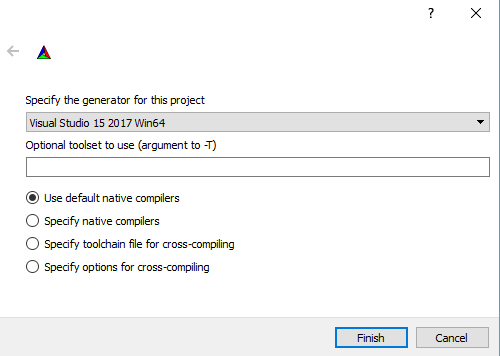
\includegraphics[width=0.5\textwidth]{tuto1}
			\item Appuyer sur "Configure"
			\item Sélectionner "Visual Studio 15 2017 Win64" en tant que "générateur" \\
				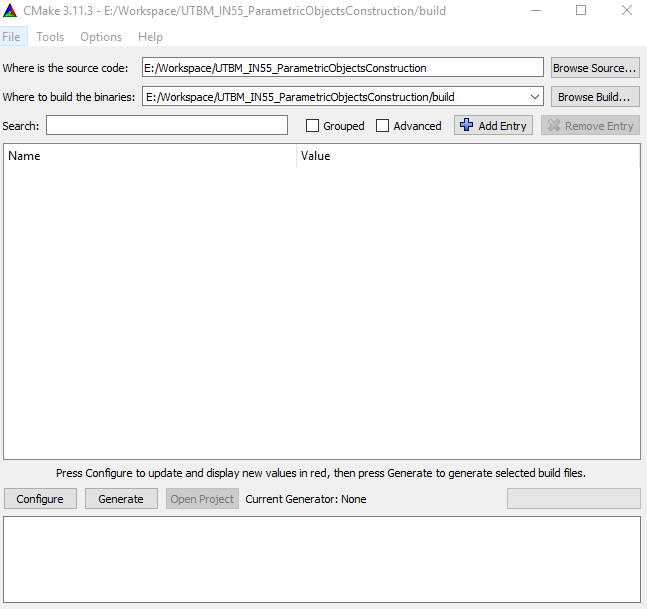
\includegraphics[width=0.5\textwidth]{tuto2}
			\item Appuyer sur "Finish"
			\item Une fois la configuration générée, appuyer sur "Generate"
			\item Appuyer sur "Open Project"
			\item Sélectionner "ParametricObjectsConstruction" comme projet de démarrage (dans l'explorateur de solution) en appuyant sur "Définir comme projet de démarrage" \\
				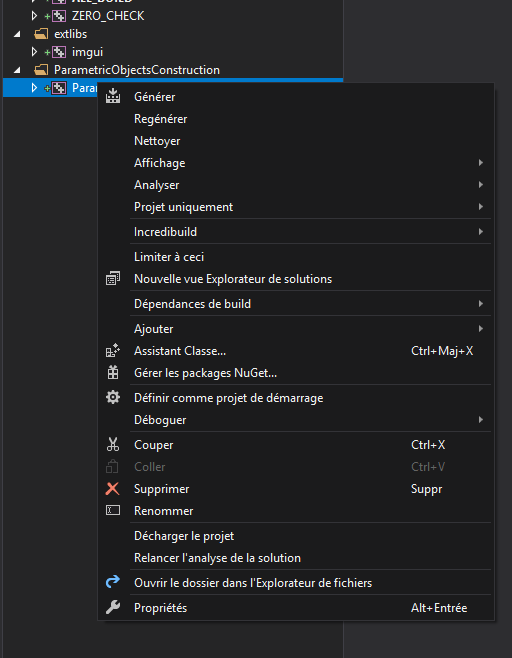
\includegraphics[width=0.5\textwidth]{tuto3}
		\end{itemize}

		\subsection{Utilisation}
			Afin de modifier l'objet paramétrique, on pourra utiliser le menu disponible sur la gauche du programme~: \\
			\begin{minipage}[t]{0.4\textwidth}
				\begin{figure}[H]
					\centering%
					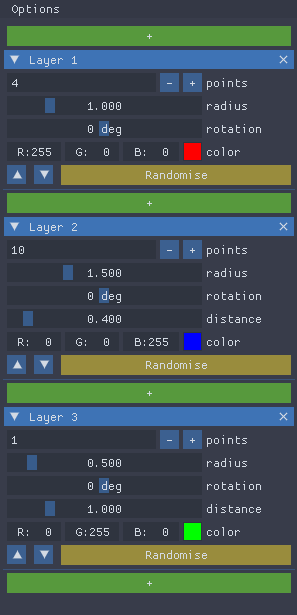
\includegraphics[width=0.7\textwidth]{menu}%
					\caption{Menu de configuration}%
					\label{fig:menu}%
				\end{figure}
			\end{minipage}
			\begin{minipage}[t]{0.59\textwidth}
				\begin{figure}[H]
					Dans ce programme les objets seront construits en utilisant des Layers. \\
					\hfill \\
					Chaque Layer correspond à un cercle sur lequelle on placera des points. \\
					\hfill \\
					La taille du cercle ainsi que le nombre de points peuvent être choisis dans le menu. \\
					\hfill \\
					Le paramètre distance permet d'éloigner un layer par rapport au layer précédent \\
					\hfill \\
					Enfin on pourra rajouter, supprimer ou réordonner les layers.
				\end{figure}
			\end{minipage}
	\section{TODO}
		\TODO{TODO}
		\par\noindent\begin{minipage}[t]{\textwidth}
			\centering
			\begin{minipage}[t]{0.49\textwidth}
				\begin{figure}[H]
					\centering%
					\resizebox{\textwidth}{!}{\import{figures/}{layers_1_empty.tex}}%
					\caption{Layers no liés}%
					\label{fig:layers_1_empty}%
				\end{figure}
			\end{minipage}
			\begin{minipage}[t]{0.49\textwidth}
				\begin{figure}[H]
					\centering%
					\resizebox{\textwidth}{!}{\import{figures/}{layers_2_nearest_lines.tex}}%
					\caption{Liaison avec les points les plus proches}%
					\label{fig:layers_2_nearest_lines}%
				\end{figure}
			\end{minipage}
		\end{minipage}
		\TODO{TODO}
		Comme illustré sur la figure \ref{fig:layers_1_empty}\ldots
		\par\noindent\begin{minipage}[t]{\textwidth}
			\centering
			\begin{minipage}[t]{0.49\textwidth}
				\begin{figure}[H]
					\centering%
					\resizebox{\textwidth}{!}{\import{figures/}{layers_3_triangles_quadrilaterals.tex}}%
					\caption{Délimitation de triangles et quadrilatères}%
					\label{fig:layers_3_triangles_quadrilaterals}%
				\end{figure}
			\end{minipage}
			\begin{minipage}[t]{0.49\textwidth}
				\begin{figure}[H]
					\centering%
					\resizebox{\textwidth}{!}{\import{figures/}{layers_4_quadrilaterals_diagonals.tex}}%
					\caption{Coupure des quadrilatères sur la diagonale la plus courte}%
					\label{fig:layers_4_quadrilaterals_diagonals}%
				\end{figure}
			\end{minipage}
		\end{minipage}
		\TODO{TODO}
		\par\noindent\begin{minipage}[t]{\textwidth}
			\centering
			\begin{minipage}[t]{0.49\textwidth}
				\begin{figure}[H]
					\centering%
					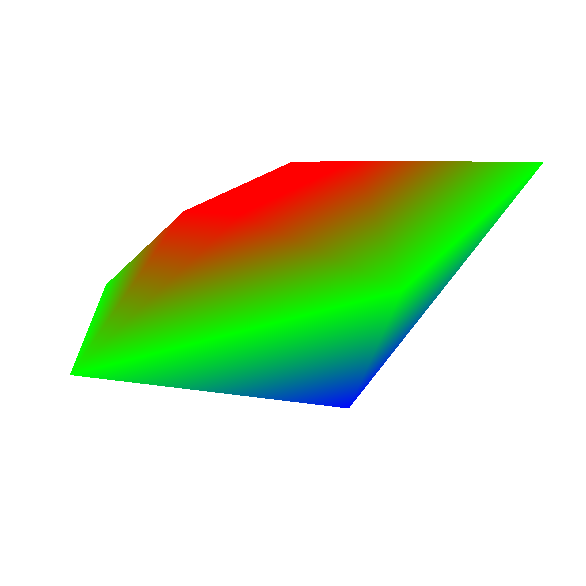
\includegraphics[width=1\textwidth]{view_1_1}%
					\caption{Exemple: vu de coté}%
					\label{fig:view_1_1}%
				\end{figure}
			\end{minipage}
			\begin{minipage}[t]{0.49\textwidth}
				\begin{figure}[H]
					\centering%
					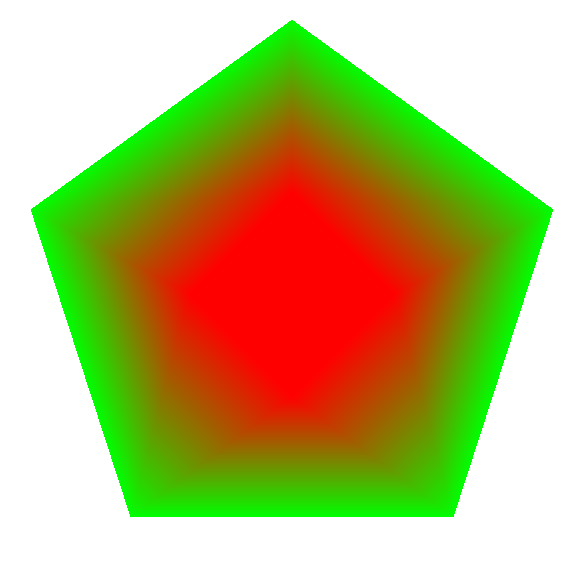
\includegraphics[width=1\textwidth]{view_1_2}%
					\caption{Exemple: vu du dessus}%
					\label{fig:view_1_2}%
				\end{figure}
			\end{minipage}
		\end{minipage}
		\TODO{TODO}
\end{document}
